\begin{frame}[allowframebreaks]{So far...}
You've practiced with on-premises solutions

Open questions?
\i How do we set up independent services?
\i How do we integrate such services?
\i How do we interface the services?

Let's guess
\i How would you do that?
\i How much time would it take?

\framebreak

No easy answers

Big-data (distributed) architectures require \textit{a lot} of skills
\i installation: how do i cable dozens cluster?
\i management: how do i replace a broken disk?
\i installation: how do i set up a new machine?
\i upgrade: how do i extend the cluster with new services/machines?
\i (energy and cooling, networking, software licenses, insurance...)

\framebreak

Technological perspective
\i it depends on your (team) skills (not only software engineering)
\si how do we orchestrate data flows?
\si how do control resource accesses (e.g., storage)?
\si how do we configure a distributed environment?

Business perspective
\i no free lunch, each choice as cost/benefit
\si how much time does it take to master a technology?
\si how many people do i need?

\framebreak

Can we afford to spend resources on tasks are not core for our mission?
\i mission: a statement used by a company to explain its purpose(s)

How can I build a working application/data platform?

\end{frame}

\sec{Cloud computing and big data}

\ssec{Why going cloud}

\begin{frame}
\includegraphics[width=\textwidth]{imgs/xkcd_cloud.png}
\end{frame}

\begin{frame}{Definition}
\begin{block}{Cloud computing (National Institute of Standards and Technology, NIST)}
A model for enabling ubiquitous, convenient, on-demand network access to a shared pool of configurable computing resources (e.g., networks, servers, storage, services) that can be rapidly provisioned and released with minimal management effort or service provider interaction. 
\end{block}

\i On-demand self-service (consume services when you want)
\i Broad network access (consume services from anywhere)
\i Resource pooling (infrastructure, virtual platforms, and applications)
\i Having big pools of resources enables economy of scale
\i Rapid elasticity (enable horizontal scalability)
\i Measured service (pay for the service you consume as you consume)
\end{frame}

\begin{frame}[allowframebreaks]{Why going cloud?}
\textbf{Scalability} that is not possible on premises
\si scale from one server to thousands
of servers
\si grow storage from gigabytes to petabytes
\si no longer think about rack space, switches, and power supplies

\textbf{Reliability} 
\i built to handle failures
\i fault-tolerant or highly available

\framebreak

\textbf{Resource pooling}
\i enable a resource to serve different consumers
\i dynamically assigned and reassigned according to demands
\i economy of scale

\textbf{Elasticity}
\i automated ability to scale resources in response to run-time conditions
\i core justification for the adoption of cloud

\framebreak

Worldwide \textbf{deployment}
\i deploy applications as close to customers as possible
\i improve data locality and privacy

Service \textbf{integration}
\i services solve common problems (e.g., load balancing, queuing)
\i do not reinvent the wheel

User perspective
\i eliminate repetitive tasks to focus on strategic ones
\i adapt infrastructure to requirements, create (test) environments on demand
\i abstract the underlying architecture

\framebreak

Service \textbf{integration} and \textbf{abstraction} are drivers of change
\i From databases to data plaforms
\i From on-premises hardware to serverless architectures

\end{frame}

\sssec{Data platform}
\begin{frame}[allowframebreaks]{Data platform}

Companies are collecting huge volumes of data to enable advanced analytics 
\i Data are more and more heterogeneous and complex
\i Databases/warehouses are no  longer ideal data hubs for integration/analysis

However, 
\i Raw data are difficult to obtain, interpret, describe, and maintain
\i There is a need for describing/curating the data to make them consumable

Data lakes (DLs) have increasingly taken the role of such hubs
\i Eliminate up-front costs of ingestion since data are stored in original format
\i Once in DL, data are available for analysis by everyone in the organization

\framebreak

However, 
\i getting  value  from  data  is  not  only  a  matter of storage
\i need integrated and multilevel analytical skills and techniques

Couto et al.: \textit{"A DL is a \b{central} repository system for \r{storage, processing, and analysis} of raw data, in which the data is kept in its original format and is \g{processed to be queried only when needed}.  It can store a varied amount of formats in big data ecosystems, from unstructured, semi-structured, to structured data sources."}

\framebreak

Drawing a sharp line been storage/computation/analysis is hard
\i Is a database just storage?
\i What about SQL?
\i What about OLAP?

Blurring of the architectural borderlines
\i ``DL'' is often replaced by ``data platform'' or ``data ecosystem''
\i encompass systems supporting data-intensive storage, computation, analysis

(Cloud-based) Data platform (e.g., Google and Amazon)
\i rationale: relieve users from complexity of administration and provision
\si not only technological skills, but also privacy, access control, etc.
\si only focus on functional aspects

\framebreak

Are we done? No!
\i lacking smart support to govern the complexity of data and transformations
\i data transformations must be governed to prevent DP turns into a swamp
\si amplified in data science, with data scientists prevailing data architects
\si leverage descriptive metadata and maintenance to keep control over data

\framebreak

Data provenance\footnote{\emph{Data provenance} and \emph{data lineage} are used in the literature as synonyms or with slightly-different flavors}
\i metadata pertaining to the history of a data item
\i pipeline including the origin of \textbf{objects} and \textbf{operations} they are subjected to
\i we have a standard: \url{https://www.w3.org/TR/prov-dm/}

\begin{figure}
    \centering
    \includegraphics[width=.5\linewidth]{imgs/prov.PNG}
\end{figure}

\framebreak

Data quality
\i Monitoring of the quality (e.g., accuracy) of the objects produced
\i notify when a transformation pipeline is not behaving as expected

Debugging 
\i Inferring the cause of pipeline failures is challenging
\i Store inputs of each operation along with 
\si their versions
\si environmental settings (e.g., RAM and CPUs)

And so on...

\framebreak

Are we done? no!
\i metadata can become bigger than data themselves
\i we need meta meta-data (or models)...
\i ... chasing our own tails
\end{frame}

\sssec{From PaaS to FaaS (serverless)}
\begin{frame}[allowframebreaks]{From PaaS to FaaS (serverless)}

Cloud services are hosted in multiple locations worldwide
\i Locations are composed of regions and availability zones
\i Each region has multiple availability zones. 
\si Each region is a separate geographical area
\si Each region is completely independent
\si Availability zones in a region are connected through low-latency links
\si Resources are usually replicated across zones but not regions

\framebreak

%\begin{frame}{Types of cloud}
\begin{figure}
    \centering
    \includegraphics[height=.5\textheight]{imgs/cloud_types.png}
\end{figure}
\i Public: accessible to anyone willing to pay (e.g., Microsoft, AWS, Google)
\i Private: accessible by individuals within an institution
\i Hybrid: a mix of the previous

%\end{frame}
\framebreak
%\begin{frame}{Cloud providers}

\begin{figure}
    \centering
    \includegraphics[height=.8\textheight]{imgs/cloud_providers.png}
\end{figure}

%\end{frame}
\framebreak
% \begin{frame}{Types of cloud}

\begin{figure}
    \centering
    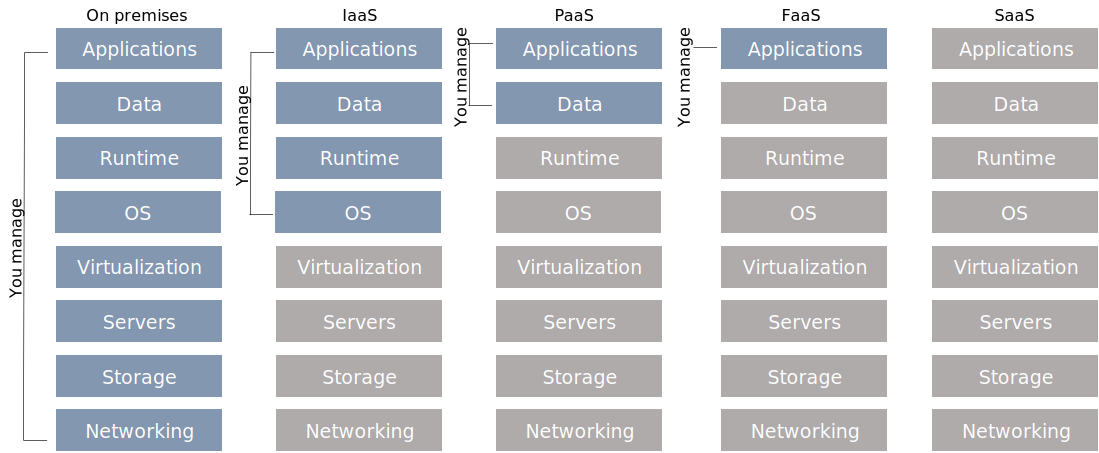
\includegraphics[height=.6\textheight]{imgs/cloud_paastosaas.pdf}
\end{figure}

%\end{frame}
\framebreak
%\begin{frame}[allowframebreaks]{Types of cloud}

Understanding architectures is paramount to successful software systems
\i good architectures help to scale
\i poor architectures cause issues that necessitate a costly rewrite

\textbf{On premises}
\i provisioning, managing, and patching servers is time-consuming
\i require dedicated operations people
\i a non-trivial environment is hard to set up and operate effectively
\i infrastructure and hardware are often a distraction from strategic tasks

\framebreak

\textbf{Infrastructure as a service (IaaS)} 
\i a computing infrastructure provisioned and managed over the internet
\i avoid expense/complexity of buying/managing \textit{physical} servers/data-centers
\i IaaS overcomes issues on premises
\si possibly requires to manage many environments

\textbf{Platform as a Service (Paas)}
\i a development and deployment environment in the cloud
% \i like IaaS, includes infrastructure-servers, storage, and networking
\i support complete application life-cycle: building, testing, deploying, etc.
\i avoid expense/complexity of managing licenses and application infrastructure

\framebreak

\textbf{Function as a Service (FaaS)}
\i a coding environment, cloud provider provisions platform to run the code
\i infrastructure provisioning and management are invisible to the developer
\i avoid to manage infrastructure

\textbf{Software as a service (SaaS)} 
\i an application environment 
\i access cloud-based apps over the Internet (e.g., email, Microsoft Office 365)
%\end{frame}
\framebreak
% \begin{frame}[allowframebreaks]{From PaaS to FaaS (serverless)}

\textbf{PaaS} and \textbf{containers} are potential solutions to inconsistent infrastructures

\i \textbf{PaaS} provides a platform for users to run their software
\si developers write software targeting features/capabilities of the platform

\i \textbf{containerization} isolates an application with its own environment
\si lightweight alternative to full virtualization
\si containers are isolated but need to be deployed to (public/private) server
\si excellent solution when dependencies are in play
\si "housekeeping" challenges and complexities

% \begin{block}{Microservices}
% Small, standalone, fully independent services built for a specific purpose
% \end{block}
% \i Each service written in an appropriate framework and language
% \si Benefits from the right language/libraries
% \si Many languages and frameworks are hard to support
% \i Each microservice can maintain state and store data
% \si eventual consistency, transaction management, and complex error recovery can make things hard

\framebreak


\textbf{Serverless}
\i a software architecture that does not rely on direct access to a server

FaaS is based on a serverless approach
\i every function could be considered as a standalone service
\i embodies principles from microservices
\si small, standalone, fully independent services built for a specific purpose
\si each service written in an appropriate framework and language
\i cloud provider is responsible for integration 
% \i Many languages and frameworks are hard to support
% \i Each microservice can maintain state and store data

\framebreak

Principles of FaaS/serverless architectures
\i use a compute service to execute code on demand (no servers/containers)
\i write single-purpose stateless functions
\i functions react to events
\si design push-based, event-driven pipelines
\i create thicker, more powerful front ends
\i embrace third-party services
\i security is designed for each function

\framebreak

Write single-purpose stateless functions
\i keep the single responsibility principle in mind
\si a function that does just one thing is more testable and robust
\si a function with a well-defined interface is also more likely to be reused
\i code should be created in a stateless style
\si local resources or processes will not survive along sessions
\si statelessness allows scalability
\i functions that terminate sooner are cheaper 
\si (pricing is based on \#requests, execution time, and allocated memory)
% Having less to do in Lambda is cheaper.  Moreover, building a rich front end (in lieu of a complex back end) that can talk to third-party services directly can be conducive to a better user experience. Fewer hops between online resources and reduced latency will result in a better perception of performance and usability of the application. In other words, you don’t have to route everything through a compute service. Your front end may be able to communicate directly with a search provider, a database, or another useful API.

Compose functions in a loose orchestration
\i build complex but understandable back-end systems
\i event-driven and push-based pipelines

\framebreak

FaaS/Serverless is not a silver bullet
\i not appropriate for latency-sensitive applications 
\i strict specific service-level agreements
\i vendor lock-in can be an issue for enterprise and government clients
\i should not base mission-critical applications on a public cloud
\i Lock-in issues
\i Migration

% TODO: Migration to cloud: pattern prevedibile? carico di lavoro? quantità dati? CPU? RAM? sposto tutto AS IS? Oppure posso ottimizzare? EMR (cluster EC2 vs cluster Kubernetes). Gestito = sicurezza + isntallazione + monitoring, logging

\end{frame}

% \begin{frame}{History in (very) brief}
% Computing as a service is far from new

% \begin{itemize}
% \item 1961, John McCarthy at MIT: "Computing may someday be organized as a public utility just as the telephone system [...] Each subscriber needs to pay only for the capacity he uses, but he has access to all programming languages characteristic of a very large system" 
% \item 1969, UCLA turns on first node of ARPANET. "As [computer networks] grow up and become more sophisticated, computer utilities will spread"
% \item 1990s USA, gigabit testbeds linked research laboratories. "Meta-computer", virtual computational systems created by linking components at different sites
% \item Large Hadron Collider (LHC) federates computing systems at hundreds of sites to analyze PBs of data. LHC Computing Grid enables on-demand access to computing and storage 
% % 2006 Emergence of cloud computing, a story of marketing, business model, and technological innovation
% % \i Cloud is driven by a transformation in demand (First successful IaaS emerged from an e-commerce provider)
% % \i Amazon was building hundreds of similar work-unit computing systems to support different services
% \end{itemize}
% \end{frame}
% \begin{frame}{Data transformation}
% 
\includegraphics[height=.8\textheight]{imgs/knowledgepyramid.pdf}
% \end{frame}


\ssec{Data pipelines on cloud}

\begin{frame}{}
\includegraphics[width=\linewidth]{imgs/xkcd_pipeline.png}    
\end{frame}

\begin{frame}{Date pipelines on cloud}
Architecting data pipelines on cloud requires to \textbf{standardize/integrate} services
\i Make them available through simple portals
\i Track usage/cost with billing mechanism
\i Measure availability
\i Orchestrate to meet demand
\i Provide a security framework
\end{frame}

\begin{frame}{Which services do we need?}
\begin{figure}
\centering

\includegraphics[height=.7\textheight]{imgs/knowledgepyramid.pdf}
\end{figure}
\end{frame}

\begin{frame}[allowframebreaks]{A tentative organization}
\begin{figure}
\centering
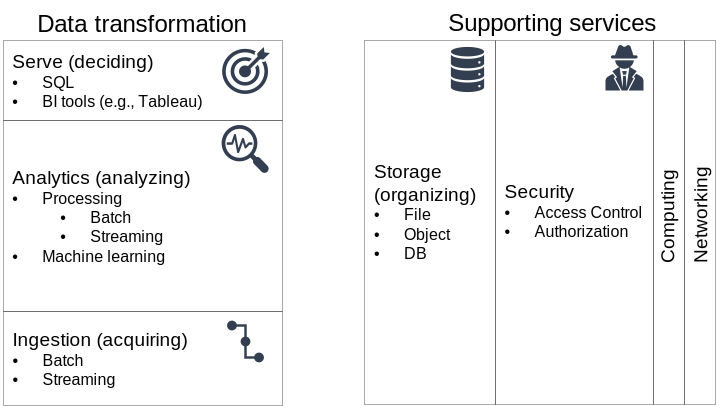
\includegraphics[height=.7\textheight]{imgs/cloudpatchwork.pdf}
\end{figure}

\framebreak

Not a sharp taxonomy

Ingestion vs Analytics
\i Data streams are used for ingestion
\i ... and (event) processing

Storage vs Database 
\i Databases are storage
\i ... with processing capability
\i ... and with serving capability

\framebreak

Categorizing features (the big-data cube \cite{meijer2012your})
\begin{columns}
\begin{column}{0.5\textwidth}
\begin{itemize}
\item Volume: small to high
\item Variety: structure to unstructured
\item Velocity: pull to push
\end{itemize}
\end{column}
\begin{column}{0.5\textwidth}
\begin{figure}
\centering
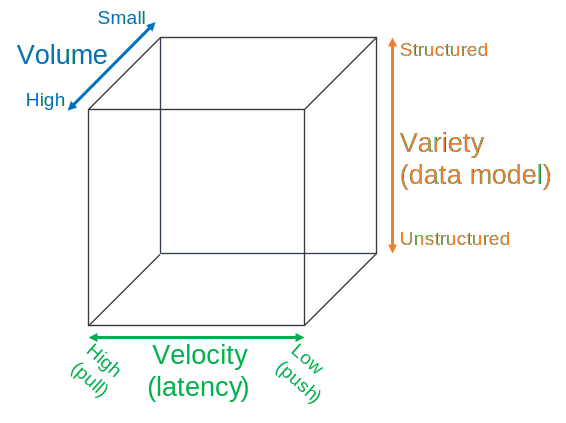
\includegraphics[scale=.4]{imgs/bigdatacube.pdf}
\end{figure}
\end{column}
\end{columns}

\framebreak

\begin{columns}
\begin{column}{0.5\textwidth}
Volume
\begin{itemize}
\item Small: small relational DBs
\item High: TBs o PBs of data
\end{itemize}
\end{column}
\begin{column}{0.5\textwidth}
\begin{figure}
\centering
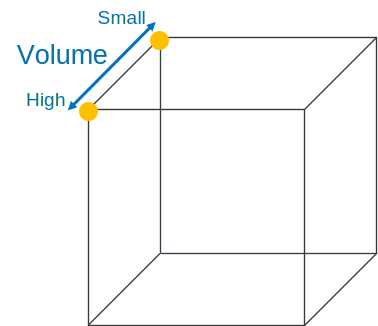
\includegraphics[scale=.4]{imgs/bigdatacube1.pdf}
\end{figure}
\end{column}
\end{columns}

\framebreak

\begin{columns}
\begin{column}{0.5\textwidth}
Variety
\begin{itemize}
\item structured: relational tuples with FK/PK relationships
\item unstructured
\begin{itemize}
    \item key-value
    \item columnar
    \item document-based
    \item graph
\end{itemize}
\end{itemize}
\end{column}
\begin{column}{0.5\textwidth}
\begin{figure}
\centering
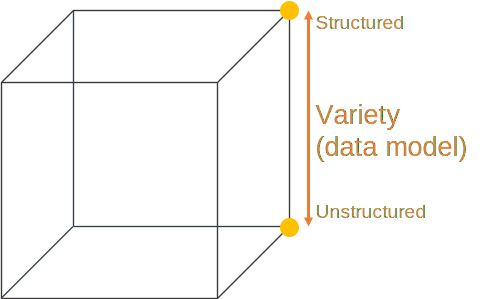
\includegraphics[scale=.4]{imgs/bigdatacube2.pdf}
\end{figure}
\end{column}
\end{columns}

\framebreak

\begin{columns}
\begin{column}{0.5\textwidth}
Velocity (latency)
\begin{itemize}
\item high: clients synchronously pulling data from sources 
\item low: sources asynchronously pushing data to clients
\end{itemize}
\end{column}
\begin{column}{0.5\textwidth}
\begin{figure}
\centering
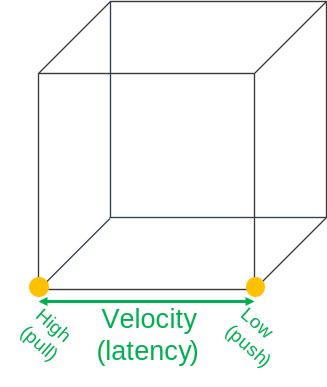
\includegraphics[scale=.4]{imgs/bigdatacube3.pdf}
\end{figure}
\end{column}
\end{columns}

\framebreak

\begin{columns}
\begin{column}{0.5\textwidth}
Our focus (in this course)
\begin{itemize}
\item (un)structured big-data batch
\item (un)structured big-data streams
\end{itemize}

\textbf{Goal}: keep in mind the cube to categorize the following services
\end{column}
\begin{column}{0.5\textwidth}
\begin{figure}
\centering
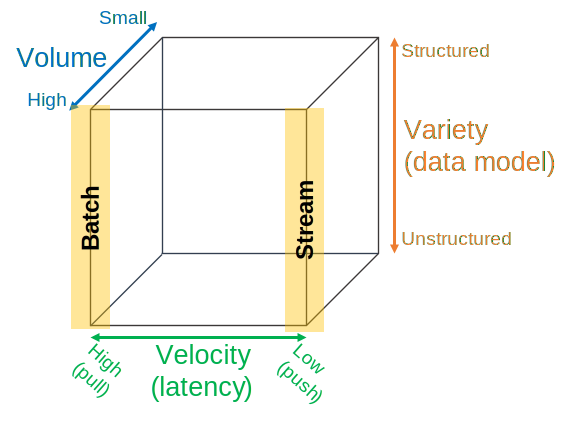
\includegraphics[scale=.4]{imgs/bigdatacube4.pdf}
\end{figure}
\end{column}
\end{columns}

% \framebreak

% \begin{figure}
%     \centering
%     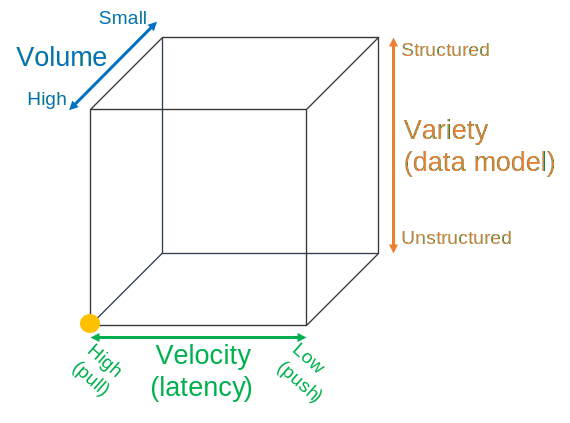
\includegraphics[scale=.4]{imgs/bigdatacube5.pdf}
% \end{figure}

% \framebreak

% \begin{figure}
%     \centering
%     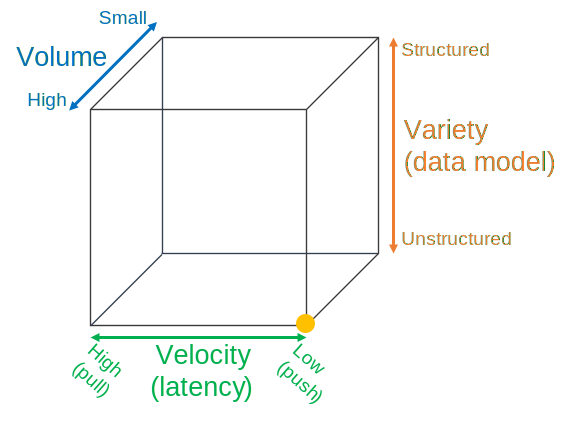
\includegraphics[scale=.4]{imgs/bigdatacube6.pdf}
% \end{figure}

% \begin{frame}[allowframebreaks]{At what costs?}
% Physical costs (and economy of scale)
% \si charges for AWS have been reduced 42 times since 2008 (up to 2014)
% \si 12/2014, charges for outbound data transfer were lowered by up to 43\%
% \si 11/2014, charges for search service were lowered by 50\%
% \si 03/2014, charges for virtual server were lowered by up to 40\%


% However, datasets are
% \i From various sources and unstructured (variety) 
% \i Of large size (volume)
% \i With fast data in/out (velocity)

% \textbf{Challenges}: data assimilation, aggregation, classification, etc.
% \end{frame}


% \begin{frame}{Data pipeline on cloud: AWS}
% \url{https://aws.amazon.com/it/architecture/analytics-big-data}
\framebreak

AWS

\begin{figure}
    \centering
    \includegraphics[height=.7\textheight]{imgs/awspipeline.png}
\end{figure}
% \end{frame}
% \begin{frame}[allowframebreaks]{AWS: storage}\end{frame}

\framebreak

% \begin{frame}{Data pipeline on cloud: Google Cloud}
Google cloud 

\includegraphics[height=.7\textheight]{imgs/gcpipeline.png}

% AI services: pre-trained models accessible through API (e.g., transcribe)
% ML services: sagemaker, helping in training models
% Or, "low-level" frameworks (e.g., TensorFlow)
\end{frame}

\sssec{Storage}
\begin{frame}[allowframebreaks]{Storage}
\textbf{Goal}: persisting data

\textbf{Storage models}
\i Different ways in which data are organized in a storage system

Understand different storage models to choose the right one
\i Nature and size of the data
\i Analyses to be performed
\i Access/update frequencies

\framebreak
% \end{frame}

% \begin{frame}[allowframebreaks]{Storage: types of storage models}

\textbf{File system} 
\i stores unstructured binary objects in a tree of directories (folders)
\i + extremely intuitive storage abstraction
\i - no support for representing structured data
\i - hierarchical organization could not match relationships
\i - cannot navigate complex data collections
\i - need to maintain consistency as multiple processes read/write a file system

\framebreak
Amazon EFS
\i deploy FS within a specific region
\i amazon EC2 instances within that region can access that file system
\i with amazon vpc/direct connect, mount file system to on-premises machine
\i cost
\si priced by average number of gb used per month
\si if provisioned throughput, also charged by provisioned mb of throughput
\si pricing also varies according to the region

\framebreak
Google Filestore
\i deploy instances within a specific zone
\i mount fs instance in any computing instance as long as in the same network
\i cost
\si priced by gbps and by service tier (standard or premium)
\si varies according to the region

\framebreak
\begin{table}
\centering
\footnotesize
\begin{tabular}{lp{5cm}p{5cm}}
    \multicolumn{1}{c}{\textbf{Feature}} & \multicolumn{1}{c}{\textbf{Amazon EFS}} & \multicolumn{1}{c}{\textbf{Filestore}} \\
    \midrule
    Tiers/Modes & General Purpose and Max I/O. Each supports either Bursting Throughput or Provisioned Throughput mode. & Standard and premium \\
    Deployment locality & Regional & Zonal \\
    Protocol & NFSv4 & NFSv3 \\
    Encryption & Can be enabled at rest and in transit & By default, encrypted at rest and in transit \\
    Pricing & Priced by average number of GB used per month and by region of deployment. If using Provisioned Throughput mode, also priced by provisioned MB of throughput. & Priced per allocated GB per second, by region of deployment, and by service tier. \\
\end{tabular}%
\end{table}%

\framebreak

\textbf{Object Store}
\i stores unstructured binary objects (blobs, binary large object)
\i simplifies the file system model, in general supports a two-level hierarchy
\i + eliminates hierarchy 
\i + forbids updates to objects once created
\i - little support for organizing data and no support for search
\i - user must know an object's identifier to access it

\framebreak
Cloud Storage and Amazon S3
\i store objects in a bucket
\i Each object within a bucket is identified by a unique key within that bucket
\i each object has an associated metadata record
\si object size, date of last modification, and media type
\si metadata can be modified
\si add custom metadata
\i user experience for buckets is designed to be similar to that of FS
\si object keys are usually paths such as ``/foo/subdir/baz.txt''
\si provide filesystem-like APIs—for example, e.g., ``ls -R''

\framebreak
\begin{table}
  \centering
  \footnotesize
    \begin{tabular}{lp{5cm}p{5cm}}
    \textbf{Feature} & \textbf{Amazon S3} & \textbf{Cloud Storage} \\
    Unit of deployment & Bucket & Bucket \\
    Deployment identifier & Globally unique key & Globally unique key \\
    File system emulation & Limited & Limited \\
    Obj. metadata & Yes   & Yes \\
    Obj. versioning & Yes   & Yes \\
    Update notifications & Event notifications & Pub/Sub notifications for Cloud Storage, Cloud Storage triggers for Cloud Functions, and object change notifications \\
    Service classes & Standard, Standard-Infrequent Access, One Zone-Infrequent Access, Amazon Glacier* & Standard, Nearline, Coldline, Archive \\
    Deployment locality & Regional & Multi-regional and regional \\
    Pricing & Priced by amount of data stored per month, network egress, and number of common API requests & Priced by amount of data stored per month, network egress, and number of common API requests \\
    \end{tabular}%
\end{table}%

\framebreak

Access frequency/retention determine availability and pricing
\includegraphics[width=.6\linewidth]{imgs/gc_accessfrequency.png}
\i Standard: optimized for performance and high frequency access
\i Nearline: for data accessed less than once a month
\i Coldline: for data accessed less than once a quarter
\i Archive: most cost-effective, data accessed less than once a year

\framebreak
Amazon Glacier
\i Cost
\si Amount of data stored per month
\si Size of files stored
\si Retrieval type
\si Number of retrieval requests
\si Network egress
\si Storage region
\i If you delete/modify data before the minimum storage period
\si charged for the remainder of the period
\si delete an object 5 days after storing the object, charged for remaining 85

\framebreak
Cloud Storage Archive
\i Cost
\si priced by amount of data stored per month and by network egress
\si Pricing also varies by storage region
\i If you delete/modify data before the minimum storage period
\si charged for the remainder of the period

% Table generated by Excel2LaTeX from sheet 'Sheet1'
\begin{table}
  \centering
  \footnotesize
    \begin{tabular}{lp{5cm}p{5cm}}
    \textbf{First-byte latency} & \textbf{Minutes to hours} & \textbf{Milliseconds (identical to Cloud Storage Standard)} \\
    \midrule
    Retrieval types & Expedited, Standard, Bulk. Expedited users can also choose between On-Demand or Provisioned retrieval. & N/A \\
    Deployment locality & Regional & Multi-regional or regional \\
    Minimum storage period & 90 days & 365 days \\
    SLA   & No    & No \\
    Pricing & Priced by amount of data stored per month, size of files stored, retrieval type, number of retrieval requests, network egress, storage region, storage period, and number of common API requests & Priced by amount of data stored per month, network egress, storage region, storage period, and number of common API requests \\
    \end{tabular}%
\end{table}%

\textbf{Database} 
\i relational
\i NoSQL
\si key-value
\si columnar
\si document based
\si graph

\framebreak
\includegraphics[width=.8\linewidth]{imgs/gc_storage_analyses.png}

\framebreak
\begin{table}
    \footnotesize
    \centering
    \begin{tabular}{lp{5cm}p{5cm}} %p{3cm}
        \textbf{Model} & \textbf{Amazon}                                   & \textbf{Google}                        \\\hline%& \textbf{Azure} \\\hline
        Files       & Elastic File System (EFS), Elastic Block Store (EBS) & Google file system                     \\%& Azure File Storage  \\
        Objects     & Simple Storage Service (S3)                          & Cloud Storage                          \\%& Blob Storage Service\\
        Relational  & Relational Data Service (RDS), Aurora                & Cloud SQL, Spanner                     \\%& Azure SQL           \\
        NoSQL       & DynamoDB, HBase                                      & Cloud Datastore, Bigtable              \\%& Azure Tables, HBase \\
        Graph       & Titan                                                & Cayley                                 \\%& Graph Engine        \\
        Warehouse   & Redshift                                             & BigQuery                               \\%& Data Lake           \\
    \end{tabular}
\end{table}
\end{frame}

\sssec{Ingestion}
\begin{frame}[allowframebreaks]{Ingestion}
\textbf{Goal}: moving data to the cloud

Ingestion services, which are used to ingest data from a source environment into a reliable and stable target environment or data type.

Moving data to the cloud
\i \r{80TB} of data to move, \g{1Gbps} connection to the internet
\i \b{How many days}? 
\si \r{80000GB} / \g{(1Gbps / 8)} / \b{60 / 60 / 24} \~= a week without internet

\framebreak
\textbf{Batch/Bulk}
\i Move data from on-premises storage

Workflow 
\i receive shipment
\i set up
\i  transfer data
\i ship back ( shipping carrier)

\framebreak
AWS Snowball
\i AWS Snowball comes in 50TB (North America only) and 80TB versions
\i AWS Snowball is not rack-mountable
\i Throughput
\si 1 Gbps or 10 Gbps using an RJ-45 connection
\si 10 Gbps using a fiber optic connection

\framebreak
Google Transfer Appliance
\i 100TB version known as the TA100, 480TB version known as the TA480	
\i TA100 comes in a 2U rack-mountable, TA480 is not rack-mountable
\i Throughput
\si 1 Gbps or 10 Gbps using an RJ-45 connection
\si 10 Gbps using a fiber optic connection
\si 4 ethernet ports, adaptive load balancing for multi-stream throughput

\framebreak
\begin{table}
  \centering
  \footnotesize
    \begin{tabular}{lll}
    \textbf{Feature} & \textbf{AWS Snowball} & \textbf{Transfer Appliance} \\
    \midrule
    Capacity per unit & 50 TB or 80 TB & 100 TB or 480 TB \\
    \multirow{3}[0]{*}{Maximum transfer rate} & \multirow{3}[0]{*}{10Gbps} & 20Gbps for TA100 \\
    \multicolumn{1}{l}{} & \multicolumn{1}{l}{} & 40Gbps for TA480 \\
    \multicolumn{1}{l}{} & \multicolumn{1}{l}{} & Both with automatic link aggregation \\
    Email status updates? & No    & Yes \\
    \multirow{2}[0]{*}{Rack-mountable?} & \multirow{2}[0]{*}{No} & Yes for TA100 \\
    \multicolumn{1}{l}{} & \multicolumn{1}{l}{} & No for TA480 \\
    \multirow{2}[0]{*}{Use fee} & \$200 for 50 TB & \$300 for TA100 \\
    \multicolumn{1}{l}{} & \$250 for 80 TB & \$1800 for TA480 \\
    \multirow{2}[0]{*}{Daily fee} & \multirow{2}[0]{*}{\$15/day after 10 days} & \$30/day after 10 days for TA100 \\
    \multicolumn{1}{l}{} & \multicolumn{1}{l}{} & \$90/day after 25 days for TA480 \\
    Transfer modes & Push  & Push or pull \\
    Transfer data out of object store? & Yes   & No \\
    \end{tabular}%
\end{table}%

\framebreak
\textbf{Stream}
\i Real-time streaming data 

% \ssec{Event streams}
% \begin{frame}{Key concepts}

\textbf{Event}: anything that we can observe occurring at a particular point in time

\textbf{Continuous streaming}: an illimitated succession of individual events, ordered by the point in time at which each event occurred

\textbf{Publish/subscribe (pub/sub)}: a way of communicating messages

\i Senders publish messages associated with one or more topics
\i Receivers subscribe to specific topics, receive all messages with that topic
\i Messages are events
% \end{frame}

\framebreak
% \begin{frame}{The unified log}

\begin{block}{Unified log}

Unified, append-only, ordered, distributed log that allows the centralization of continuous event streams

\end{block}

General idea:

\i Collect events from disparate source systems
\i Store them in a unified log
\i Enable data processing applications to operate on these event streams
% \end{frame}

\framebreak
% \begin{frame}{Features of a unified log}

\textbf{Unified}: a single deployment of this technology a company, with multiple applications sending events to it and reading events from it
  \i Log serves as central data backbone
  \i Unified log can contain many distinct continuous streams of events
  \si Not all events are sent to the same event stream

\textbf{Append-only}: new events are appended to the unified log
\i existing events are never updated in place
\i if read the event \#10, never look at events 1 through 10 again
\i Events are automatically deleted from the unified log when they age 
% \end{frame}

\framebreak
% \begin{frame}{Features of a unified log}
\textbf{Distributed}: the unified log lives across a cluster of machines

\i Still, the log is unified since we have a single (conceptual)
\i Scalability: work with streams larger than the capacity of single machines
\i Durability: replicate all events within the cluster to overcome data loss
\i Divide events in a given stream into *shards* (partitions)

\includegraphics[width=.6\linewidth]{imgs/eventstream_shard.jpg}
% \end{frame}

% \begin{frame}{Features of a unified log}
\textbf{Ordered}: events in a shard have a sequential IDs (\textit{offset}, unique within a shard)
\i Local ordering keeps things much simpler
\i Applications maintain their own cursor for each shard

\includegraphics[width=.4\linewidth]{imgs/eventstream_order.jpg}
% \end{frame}

\framebreak
% \begin{frame}[allowframebreaks]{Event stream processing}
Two types of processing can be performed on a single event stream
\i \textbf{Single-event}, a single event produces zero or more events
\si \textit{Validating} "Does this event contain all the required fields?”
\si \textit{Enriching} "Where is this IP address located?"
\si \textit{Filtering} "Is this error critical?"
\i \textbf{Multiple-event}, multiple events collectively produce zero or more events
\si \textit{Aggregating}, functions such as minimum, maximum, sum
\si \textit{Pattern matching}, looking for patterns or co-occurence
\si \textit{Sorting}, reordering events based on a sort key

\includegraphics[width=.8\linewidth]{imgs/eventstream_processing.jpg}
% \end{frame}

\framebreak
Amazon Kinesis Data Streams
\i streaming model to ingest data
\i producers send data to a stream that you create and provision by shard
\i each shard provides a maximum of 1 MBps and 1000 data puts per second
\i This data is stored in data records that consist of the following:
\si An incremental sequence number
\si A user-supplied partition key
\ssi load-balance records across shards
\si A data blob
\i By default, records are retained for 24 hours (maximum of 7 days)
\i Data order
\si maintains order through partition key and sequence number
\si producer provides a partition key that determines the shard
\si The shard adds an incremental sequence number to the record
\si Consumers get records by shard, records ordered by sequence number
\si ordering is not guaranteed for requests across shards
\i Operations
\si users must scale shards up and down manually
\si monitor usage with Amazon CloudWatch and modify scale as needed
\si scaling process is called resharding, 
\si split shard into two, or merge two shards
\si avoid shard management by using Kinesis Data Firehose
\ssi automate management to aggregating data into S3/Redshift
% \ssi specify S3 bucket/Redshift cluster, and Kinesis Firehose creates and manages a stream on the user's behalf, depositing the data in specified intervals into the specified location.
\i Kinesis is a regional service, with streams scoped to specific regions
\si all ingested data must travel to the region in which the stream is defined.
\i Costs
\si priced by shard hour, data volume, and data retention period
\si pay for resources you provision (even if not used)
\si Amazon Kinesis Data Firehose is priced by data volume.



\framebreak
Google Pub/Sub
\i messaging service that uses a publisher/subscriber model
\i create a Pub/Sub topic, publish data to that topic
\i applications subscribe to the topic to retrieve ingested data
\i Avoid definition of of shards.
\i push model or pull model
\si push model, the Pub/Sub server sends a request to the subscriber application at a preconfigured URL endpoint
\si pull model, the subscriber application requests messages from the server, and then acknowledges receipt
\i each data (i.e., message) must be base64-encoded and no larger than 10 MB
\si At the time of ingestion, Pub/Sub adds a messageId attribute and a publishTime
\si messageId unique within the topic
\i Data order
\si delivers messages on a best-effort basis, using system-supplied publishTime
\si does not guarantee only-once or in-order delivery: on occasion, a message might be delivered more than once, and out of order
\si subscriber should be idempotent when processing messages and able to handle messages out of order
\si achieve stricter ordering by using application-supplied sequence numbers
\i Pub/Sub does not require provisioning, and handles sharding, replication, and scaling
\si don't need to use partition keys—Pub/Sub manages data partitioning on your behalf
\si less overhead, but fewer guarantees about message ordering.
\i Pub/Sub uses Google's HTTP(S) load balancer to support data ingestion globally across all Google Cloud regions
\si load balancer automatically directs the traffic to Pub/Sub servers in an appropriate region in order to minimize latency.
\i Pub/Sub is priced by data volume
\si does not require resource provisioning, you pay for only the resources you consume

\framebreak
\begin{table}
\centering
\footnotesize
\begin{tabular}{lp{5cm}p{5cm}}
\textbf{Feature} & \textbf{Amazon Kinesis Data Streams} & \textbf{Google Pub/Sub} \\
Unit of deployment & Stream & Topic \\
Unit of provisioning & Shard & N/A (fully managed) \\
Data unit & Record & Message \\
Data source & Producer & Publisher \\
Data destination & Consumer & Subscriber \\
Data partitioning & User-supplied partition key & N/A (fully managed) \\
Retention period & Up to 7 days & Up to 7 days \\
Data delivery order & Service-supplied sequence key (best effort) & Service-supplied publish time (best effort) \\
Max data size & 1 MB  & 10 MB \\
Deployment locality & Regional & Global \\
Pricing model & Per shard-hour, PUT payload units, and optional data retention & Message ingestion and delivery, and optional message retention \\
\end{tabular}%
\end{table}%
\end{frame}

% \begin{frame}[allowframebreaks]{AWS: ingestion}
% \textbf{Batch}

% \i \textbf{AWS DataSync}
% \si move data between on-premises storage and S3/EFS/etc.
% \si on-premises software transfers data via Network File System protocol
% \si pay only for the data you copy

% \i \textbf{AWS Transfer for SFTP} 
% \si transfer files in/out Amazon S3 using Secure File Transfer Protocol




% \framebreak

% \textbf{Stream}

% \i \textbf{Kinesis} 
% \si collect, process, and analyze real-time, streaming data
% \si ingest real-time data such as video, audio, application logs, etc. 
% \si analyze data as it arrives (and not until all data is collected)

% \i \textbf{Kinesis Data Firehose}
% \si load streaming data into storage/analytics
% tools (S3, Elasticsearch, etc.)
% \si automatically scales to match the throughput

% \i \textbf{Kinesis Data Analytics}
% \si analyze streaming data in real time
% \si use SQL to continuously query streaming data
% \si scales automatically to match the volume and throughput rate

% \framebreak

% \i \textbf{Simple Queue Service (Amazon SQS)} 
% \si message queue that decouples microservices/serverless
% \si send/store/receive messages, avoid message loss
% \si \textit{Standard}: max. throughput, best-effort ordering, at-least-once delivery
% \si \textit{FIFO}: exact ordering, exactly-once delivery

% \i \textbf{Simple Notification Service (SNS)}
% \si topics for high-throughput, push-based, many-to-many messaging
% \si fan out messages to a large number of subscriber endpoints
% \end{frame}

{
\bgimg{1}{imgs/awssnowmobile.png}
\begin{frame}{AWS: ingestion}
    
\end{frame}
}





\ssec{Structural patterns for data pipelines}
\begin{frame}{Structural patterns}
Patterns are architectural solutions to problems in software design
\i Address common problems in software development
\si Command pattern
\si Messaging pattern
\si Priority queue pattern
% \si Fan-out pattern
\si Pipes and filters pattern
\end{frame}

\begin{frame}{Command pattern}
encapsulate a request as an object, thereby letting you parameterize clients with different requests, queue or log requests, and support undoable operations” because of the “need to issue requests to objects without knowing anything about the operation being requested or the receiver of the request”

\includegraphics[scale=.4]{imgs/pattern_command.PNG}
\end{frame}

\begin{frame}[allowframebreaks]{Pipes and filters pattern}
Decompose a complex processing task into a sequence of manageable services
\i Components designed to transform data are referred to as filters
\i Connectors that pass data between components are referred to as pipes

\includegraphics[width=.7\linewidth]{imgs/pattern_pipeline.PNG}
\end{frame}

\begin{frame}{Messaging pattern}
Decoupling functions and services from direct dependence on one another and allowing storage of events/records/requests in a queue. The reliability comes from the fact that if the consuming service goes offline, messages are retained in the queue and can still be processed at a later time.
\i Depending on how the system is designed, a message queue can have a single
sender/receiver or multiple senders/receivers.

\includegraphics[scale=.4]{imgs/pattern_messaging.PNG}
\end{frame}

\begin{frame}{Priority queue pattern}
Control how and when messages are dealt with
\i Different queues, topics, or streams to feed messages to your functions 
\i High-priority messages go through expensive services with more capacity

\includegraphics[scale=.4]{imgs/pattern_priority.PNG}
\end{frame}



